\documentclass[letter]{article}
\usepackage[margin=27mm, font=11pt]{geometry}
\usepackage{graphicx} % Required for inserting images
\usepackage{amsmath}
\usepackage{amsfonts}
\usepackage{amssymb}
\usepackage{booktabs}
\usepackage{hyperref}       % hyperlinks
\usepackage{url}            % simple URL typesetting
\usepackage{booktabs}       % professional-quality tables
\usepackage{nicefrac}       % compact symbols for 1/2, 
\usepackage{microtype}      % microtypography
\usepackage{xcolor}         % colors
\usepackage{graphicx}
\usepackage{dsfont}
\usepackage{dblfloatfix}
\usepackage{multicol}
\usepackage{float}
\usepackage[margin=50pt, font=small, labelfont=bf]{caption}
\usepackage{appendix}
\usepackage{makecell} % Required for \makecell command

\title{Trump (again): Individual-level logistic regression analysis of vote choice in the 2024 presidential election}
\author{Talia Fabregas}
\date{July 2025}

\begin{document}

\maketitle
\begin{abstract} Donald Trump was elected the 47th President of the United States on November 5, 2024, defeating former Vice President Kamala Harris 312 to 226 in the electoral college and 49.9\% to 48.4\% in the popular vote. This project analyzes vote choice in the 2024 U.S. Presidential Election using logistic regression and individual-level data from the 2024 Cooperative Election Study (CES). I found that including race-related interaction terms – specifically, the interactions race and gender, race and education, race and region, and race and the urban-rural divide – as well as approval of incumbent President Joe Biden and perception of the economy, prices of everyday goods, and self-reported family income changes in the past year significantly improved model fit. I trained the logistic model via minibatch gradient descent on a subset of the 2024 CES dataset and regularized it with an L2-penalty and achieved 92.8\% validation accuracy. I estimate that the interaction effects of race with demographic and geographic factors, as well as economy-related perceptions and approval of the incumbent president, significantly influenced vote choice in the 2024 election.\end{abstract}
Code and data can be found using this link: \\
\href{link}{https://github.com/taliafabs/STA496/tree/94998aba253905a6866cba4364e00de47f49eb10/MidtermPaper}
\section{Introduction}\label{sec:intro}
On November 5, 2024, Donald Trump was elected the 47th President of the United States, defeating former Vice President Kamala Harris 312 to 226 in the electoral college and 49.9\% to 48.4\% in the popular vote \cite{cnn}. President Trump won all seven key battleground states – Michigan, Wisconsin, Pennsylvania, North Carolina, Georgia, Arizona, and Nevada – by close margins. Trump is a twice-impeached, 34-time convicted felon who became the first Republican nominee to win the popular vote since former President George W. Bush in 2004. He is a one-of-a-kind president whose second victory followed an election cycle like no other. On July 21, 2024, former President Joe Biden made the unprecedented decision to end his re-election campaign. Former Vice President Harris quickly became the Democratic nominee with Biden's endorsement and ran an unprecedented 107-day campaign, the shortest in modern American history \cite{reuters}. Biden ended his re-election campaign with low approval ratings \cite{mongrain}. Top election issues included inflation, the economy, the cost of living, medicare and medicaid, and reproductive rights \cite{gallup} \cite{pew1}. \\
\\
Since then, the following question has loomed: why did Americans re-elect Trump, despite all his baggage? This paper will investigate the question of why Americans voted the way that they did on November 5, 2024. This project aims build on the works of Kuriwaki et al., Algara et al., and Camatarri by incorporating the interactions between race and education, race and region, and race and the urban-rural divide as well as voters' perception of the economy and incumbent presidential approval in a logistic regression vote choice model that focuses on individual voters \cite{kuriwaki} \cite{algara} \cite{camatarri}. Consequently, this project aims to estimate how those factors influence vote choice, with a focus on the 2024 U.S. presidential election. The estimands, which can never be known exactly, are the true effects of age, gender, race, highest level of educational attainment, state of residence, region of residence, the urban-rural divide, perception of the state of the economy, family income, and the prices of everyday goods in the year leading up to the election, and the interaction of race with region, the urban-rural divide, education and gender on presidential vote choice. Third-party presidential candidates received 1.85\% of the national popular vote in 2024, therefore my outcome of interest – 2024 presidential vote choice – is treated as binary \cite{app}. This project contributes to individual-level logistic vote choice modeling research by treating it as a binary classification task and incorporating both macro-level variables such as incumbent presidential approval and economic conditions and micro-level sociodemographic variables \cite{camatarri}. Instead of aiming to forecast an election outcome, this project aims to build and train a logistic regression model that can accurately classify likely Democratic and Republican presidential voters using the 2024 Cooperative Election Study (CES) dataset and achieve high predictive accuracy on unseen data. The Python programming language and the \texttt{numpy},  \texttt{pandas},  \texttt{scikit-learn},  \texttt{matplotlib}, \texttt{seaborn},  \texttt{statsmodels},  \texttt{TensorFlow}, and \texttt{keras} packages were used to produce the visualizations and train, fit, and evaluate the logistic models presented in this paper \cite{python}. \\
\\
The remainder of this paper is structured as follows. Section \ref{sec:lit} contains a brief discussion about the research presented by Kuriwaki et al. on race and voting behavior, Algara et al. on presidential approval and voting behavior, and Camatarri on the use of logistic regression to model individual-level voting behavior that this project aims to build on. Section \ref{sec:data} contains an overview of the 2024 Cooperative Election Study (CES) Common Content Dataset that was used to train and evaluate logistic vote choice models and exploratory data analysis findings.  Section \ref{sec:model} covers my modeling strategy and frequentist model selection process. Section \ref{sec:results} presents likelihood ratio test results and how well the selected model performed on unseen data.
\section{Literature Review}\label{sec:lit}
Existing literature shows that presidential popularity and economic conditions are significant predictors of the outcomes of presidential elections \cite{algara} \cite{camatarri} \cite{abramowitz}. In a 1988 study, Abramowitz found that the more popular an incumbent president is and the better the state of the economy, the greater the vote share for the incumbent president’s party should be, whether they are the incumbent or not \cite{abramowitz}. More recently, Camatarri built a logistic model to estimate support for Republican presidential nominees using pre-electoral waves of the ANES Time Series Study from 2012, 2016, and 2020 and found that economic disapproval was one of the strongest predictors for support of the Republican nominee when the incumbent president was a Democrat \cite{camatarri}. \\
\\
In "The Geography of Racially Polarized Voting: Calibrating Surveys at the District Level," Kuriwaki et al. performed multilevel regression with post-stratification (MRP) using 2016 Cooperative Congressional Election Study (CCES), 2020 Congressional Election Study (CES) and U.S. Census data, hierarchal modeling with calibration weights to match their estimates to aggregated vote totals, and compared their estimates with those obtained using different techniques \cite{kuriwaki}. They found that national-level racial group differences explain 60\% of differences in district-level voting behavior and that race explains voting behavior more than geography, but its influence may be declining relative to education and the urban-rural divide \cite{kuriwaki}. \\
\\
In "Partisan Collective Accountability during the 2024 US Presidential and Congressional Elections,” Algara et al. built a model to forecast four election outcomes of interest: presidential popular vote, presidential electoral college votes, number of U.S. Senate seats won by the incumbent president’s party, and number of U.S. house seats won by the incumbent president’s party using presidential approval and incumbent party brand as its two main predictors \cite{algara}. They found that presidential approval is the only key covariate that predicts the popular vote percentage and number of electoral votes won by the nominee from the incumbent president’s party \cite{algara}. This suggests that both these factors influence individual-level voting behavior. Algara et al. validated the accuracy of their forecasting model by applying it to past U.S. elections; it would have correctly predicted the electoral college winner in 15 of 21 presidential elections since 1940 \cite{algara}. Their model correctly forecasted that Harris would narrowly lose the popular vote and the electoral college to  Trump due to Biden's low presidential approval rating \cite{algara}. \\
\\
In "Predicting Popular-vote Shares in US Presidential Elections: A Model-based Strategy Relying on Anes Data," Camatarri proposes the use of standard and Bayesian logistic regression models that consider voter-level data – such as political positions, ideology, race, gender, and other socioeconomic variables – for election predictions that are based on individual-level vote choice \cite{mongrain} \cite{camatarri}. Election forecasting models that only use macro-level variables – such as economic conditions and incumbent presidential approval – aim to predict a series of many micro-level outcomes: individual voters' decisions \cite{camatarri}. Camatarri's models were tested on the 2012, 2016, and 2020 pre-electoral waves of the ANES Time Series study and 10 of the 12 models had a forecasting error below 3\% \cite{camatarri}. These results suggest that regression-based individual voter-level election models have the potential to produce accurate popular vote forecasts and compliment macro-level models \cite{camatarri}. \\
\\
Accurately classifying likely Democratic and Republican voters is a precursor for an individual-level logistic modeling approach that aims to forecast aggregate presidential election outcomes. Neither Kuriwaki et al. nor Algara et al. focus specifically on logistic vote choice modeling, but their findings highlight the influence of race on voting behavior and and the predictive power of incumbent presidential approval in forecasting election outcomes \cite{kuriwaki} \cite{algara}.
This project builds on Camatarri's approach by using existing research by including macro- and micro-level predictors in a logistic vote choice model trained on the 2024 Cooperative Election Study (CES) dataset to estimate how these factors influenced the American electorate – comprised of individual voters – to send Trump back to the White House.
\section{Data} \label{sec:data}
\subsection{Dataset overview}
The 2024 Cooperative Election Study (CES) Common Content Dataset was used for this project \cite{ces24}. The data was most recently downloaded via url from Harvard Dataverse in July 2025. The 2024 CES is an election-year wave of the CCES; it contains data from over 50,000 online interviews with American adults, conducted in the weeks leading up to and the weeks following the November 5th, 2024 presidential election \cite{ceswebsite}. The pre-election wave includes questions about general political attitudes, demographics, positions on current policies being debated in Congress, political information, and vote intentions; the post-election wave includes questions about how respondents voted in the recent election, and recent political and social engagement \cite{ces24} \cite{ceswebsite}.  Additional data preparation details are available in Appendix \ref{appendix:a}.
\subsection{Exploratory data analysis}
Exploratory data analysis findings suggest that education, race, geographic, incumbent presidential approval, and economy-related variables should be included in a logistic vote choice model. Harris voters are over-represented in the 2024 CES survey dataet. As shown in Figure \ref{fig:ces-vote_counts} the 2024 CES survey dataset is Harris +12; this is not representative of the actual results, where Trump won the popular vote by 1.5 percentage points. However, the dataset includes post-stratification weights to account for the under-representation of voters from strata associated with support for Trump \cite{ces24}. As shown in \ref{fig:ces-educ}, higher education is associated with support for Harris among 2024 CES survey respondents. \\
\\
The dataset is consistent with existing research; support for Democratic nominee Kamala Harris was higher among respondents with a favorable view of incumbent Democratic President Joe Biden and the economy \cite{algara} \cite{camatarri} \cite{ces24}. As shown in Figure \ref{fig:ces-vote_counts}, 96.5\% of respondents who believed that the economy had "gotten much better" supported Harris, while 86\% of respondents who believed that the economy had "gotten much worse" supported Trump. Respondents who believed that the economy "stayed about the same" also favored Trump over Harris (57\% vs 37.5\%) \cite{ces24}.  Almost all respondents who "somewhat approve" or "strongly approve" of the Biden administration voted Harris, while over 90\% of respondents who "strongly disapprove" of the Biden administration voted Trump \cite{algara} \cite{ces24}. \\
\\
Race remains a significant predictor of vote choice, but its effects might vary across different regions, the urban-rural divide, and highest level of educational attainment \cite{kuriwaki}. Figure \ref{fig:raceregion} shows the interaction of race and the rural-urban divide among respondents.  White respondents living in cities overwhelmingly broke for Harris and white respondents living in rural areas overwhelmingly broke for Trump. On the contrary, Black respondents living in all types of areas favored Harris \cite{ces24}. White male and female respondents had similar levels of support for Harris, but Black female respondents favored Harris more heavily than Black male respondents; this suggests that although support for Trump increased among racial minorities in 2024, white voters are still more likely to support Trump than voters of color \cite{camatarri} \cite{pew}. \cite{ces24}.
\begin{figure}[H]
    \centering
    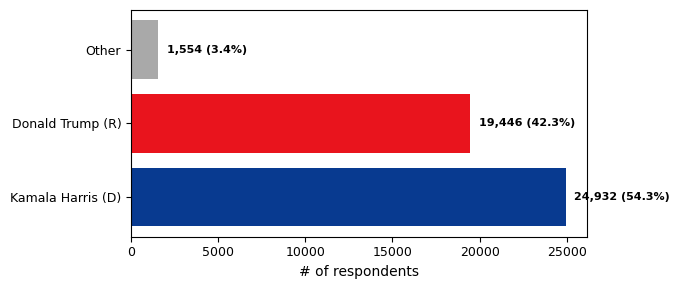
\includegraphics[scale=0.65]{eda/ces24-vote_counts.png}
    \caption{Among survey respondents, 54.3\% voted for Harris, 42.3\% voted for Trump, and 3.4\% voted third-party or write-in in the 2024 Presidential Election. }
    \label{fig:ces-vote_counts}
\end{figure} 
% race and educ
\begin{figure}[H]
    \centering
    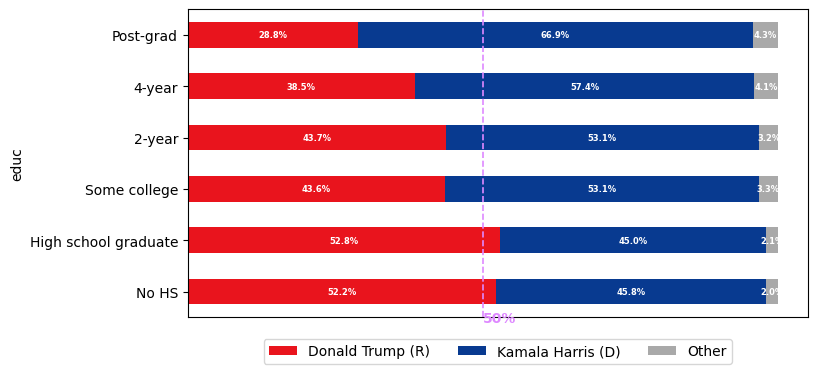
\includegraphics[scale=0.45]{eda/ces24-educ.png}
    \caption{A majority of respondents with at least some college supported Harris, with highest Harris support among respondents with a post-graduate (advanced) degree. A majority of respondents without a college education supported Trump.}
    \label{fig:ces-educ}
\end{figure} 
\begin{figure}[H]
    \centering
    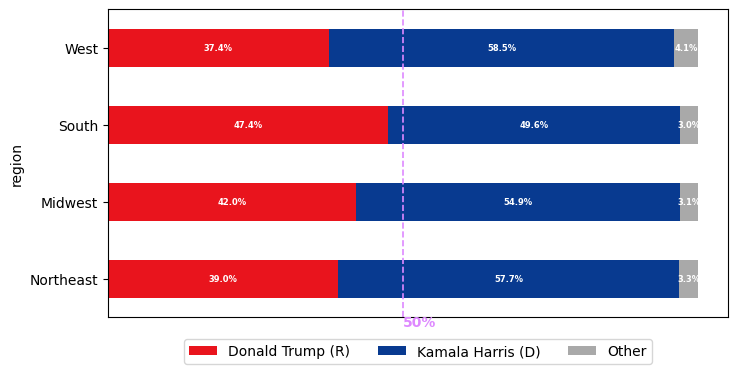
\includegraphics[scale=0.42]{eda/ces24-region.png}
    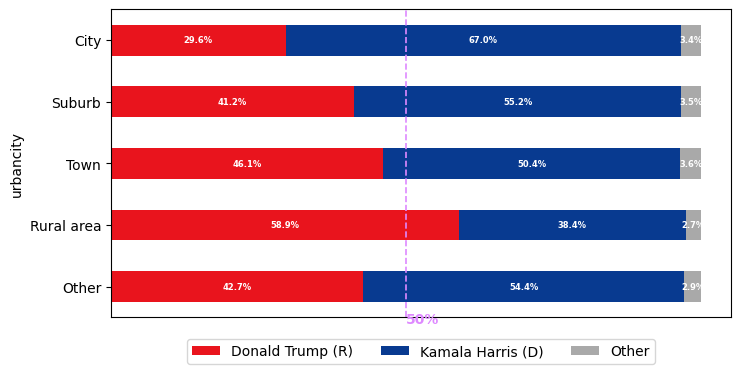
\includegraphics[scale=0.42]{eda/ces24-urban_rural_divide.png}
    \caption{Support for Harris was higher among survey respondents who live in the West, the Northeast, and in urban areas (cities and suburbs). Support for Trump was higher among survey respondents who live in the South or in rural areas/small towns.}
    \label{fig:ces-geographic}
\end{figure} 
\begin{figure}[H]
    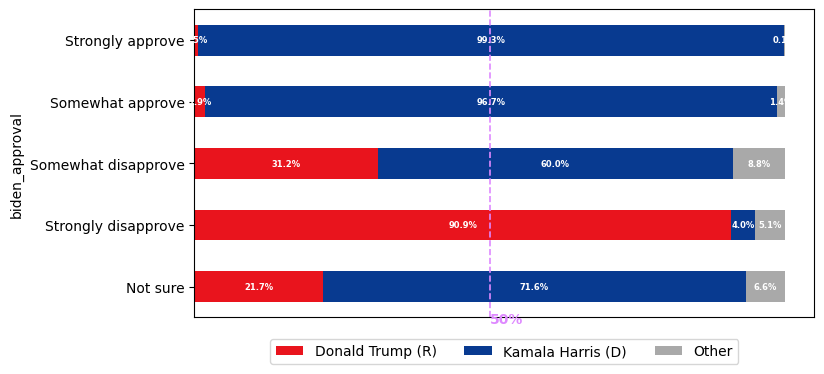
\includegraphics[scale=0.42]{eda/ces24-biden.png}
    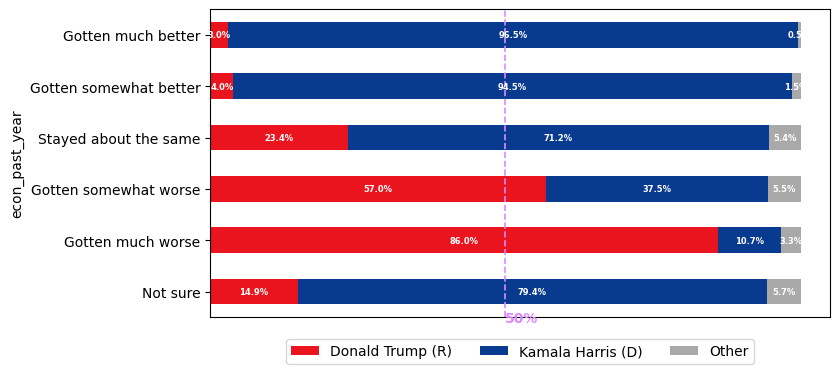
\includegraphics[scale=0.42]{eda/ces24-econ.png}
    \caption{Positive perceptions of the state of the economy in the year leading up to the 2024 presidential election and approval of the Biden administration are associated with support for Harris, while negative perceptions and disapproval of the Biden administration are associated with support for Trump among 2024 CES survey respondents.}
    \label{fig:ces-vote_counts}
\end{figure} 
\begin{figure}[H]
\centering
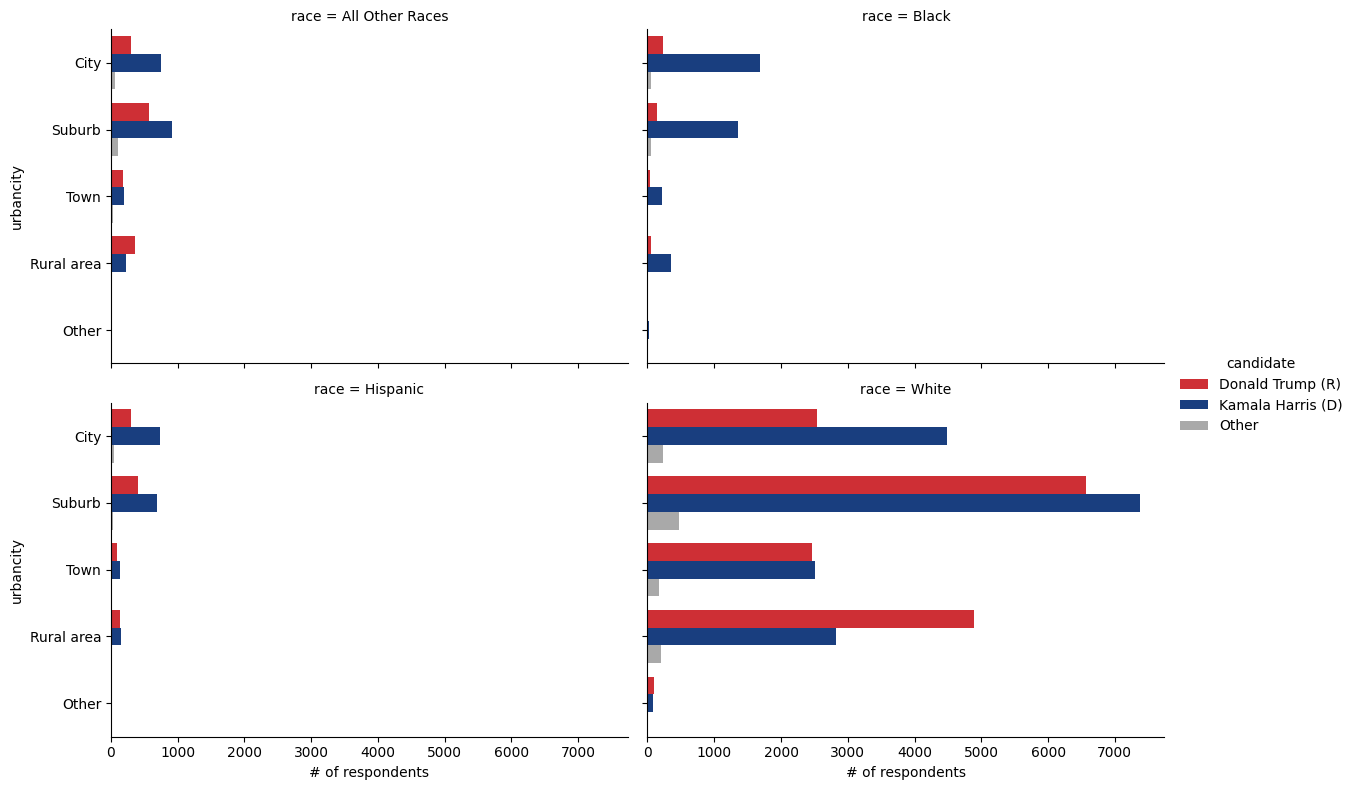
\includegraphics[scale=0.45]{eda/ces24-race_region.png}
\caption{2024 presidential vote breakdown among respondents, by race and type of area.}
\label{fig:raceregion}
\end{figure}
\begin{figure}[H]
\centering
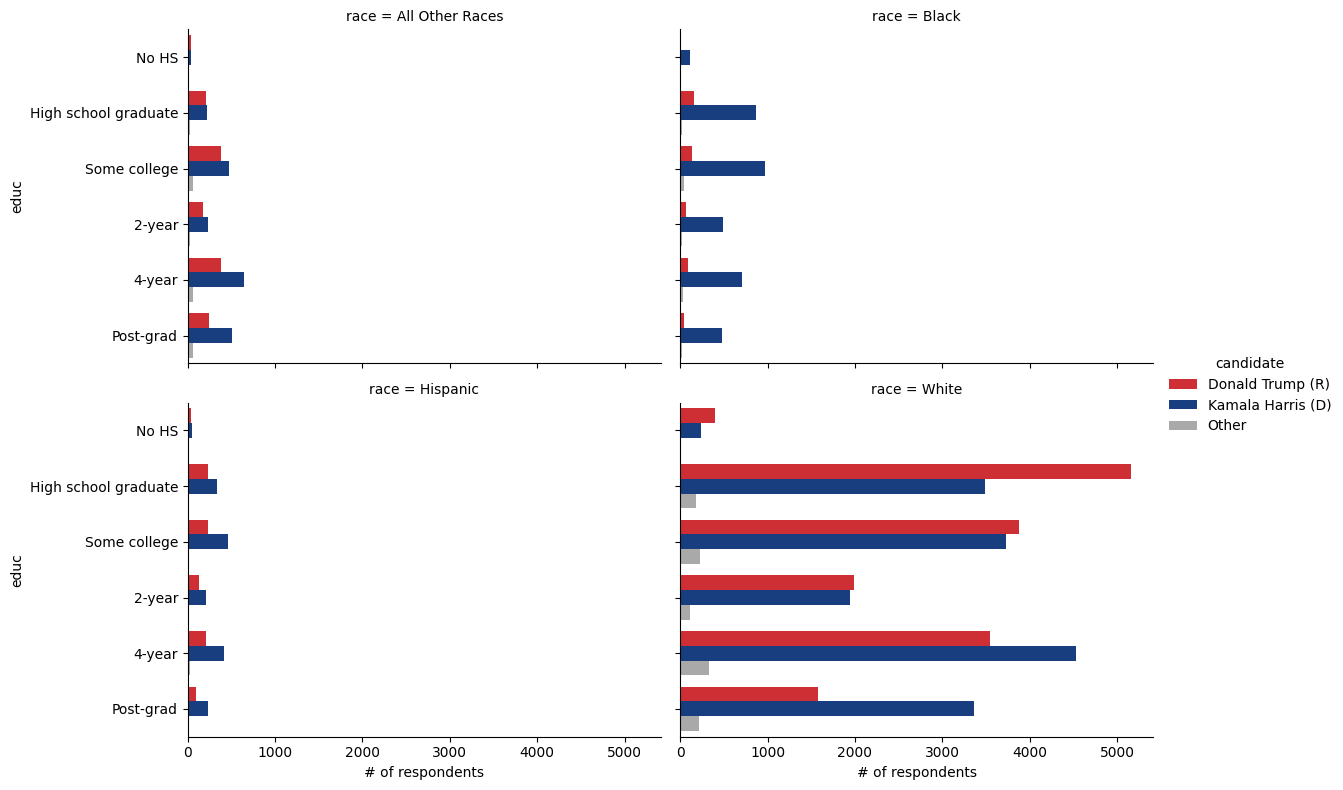
\includegraphics[scale=0.45]{eda/ces24-race_educ.png}
\caption{2024 presidential vote breakdown among respondents, by race and highest level of educational attainment.}
\end{figure}
\begin{figure}[H]
\centering
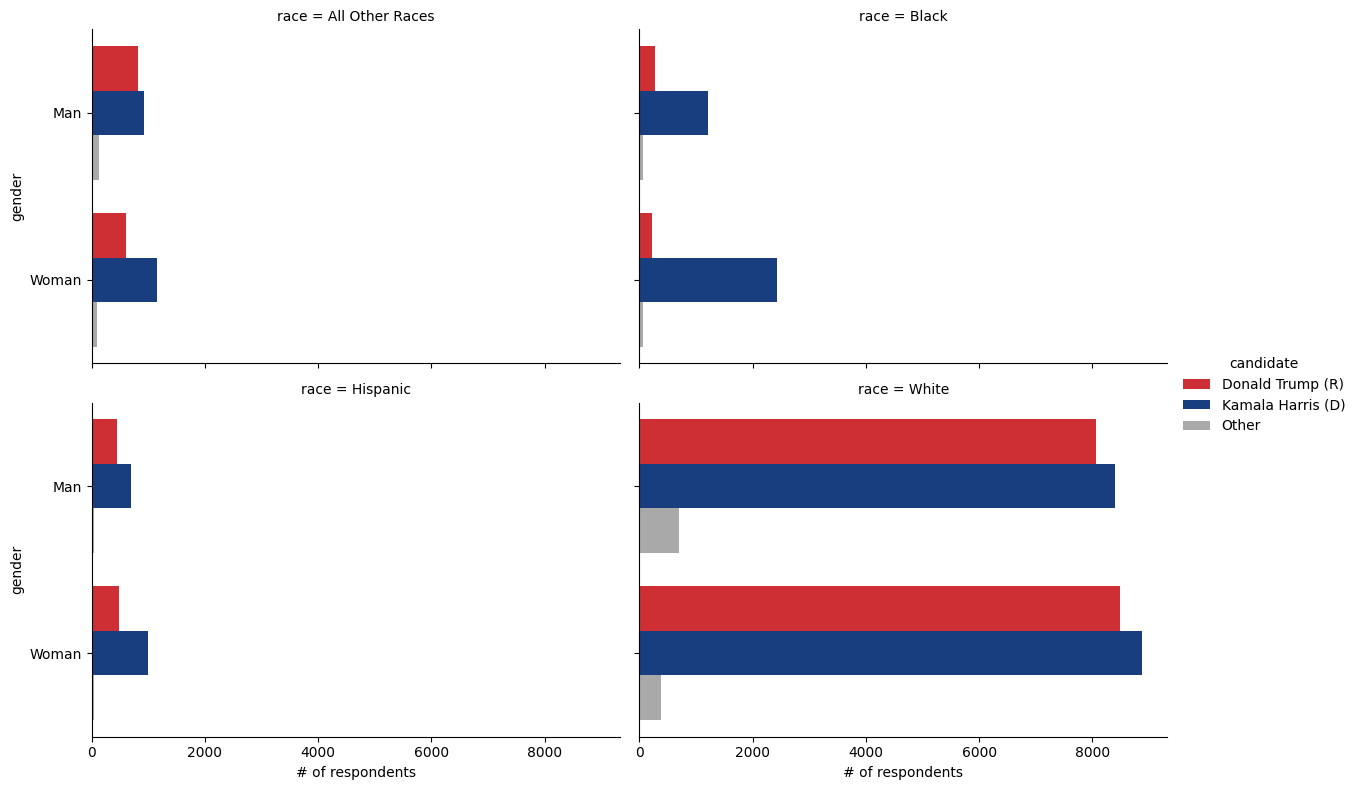
\includegraphics[scale=0.4]{eda/ces24-race_gender.png}
\caption{2024 presidential vote breakdown among respondents, by race and gender.}
\end{figure}
\section{Model} \label{sec:model}
My modeling strategy aims to identify the logistic regression model that best fits the 2024 CES survey dataset, determine which of the predictors suggested by the works of Kuriwaki et al. and Algara et al. improve model fit, and train and optimize a logistic machine learning (ML) model to accurately classify Harris and Trump voters and generalize well. Logistic regression will be used to classify respondents by vote choice because it is a simple, interpretable model suitable for predicting this binary outcome of interest \cite{camatarri}.\\
\\
Likelihood ratio testing will be used to determine which of the models outlined below best explains presidential vote choice in the 2024 CES survey dataset and whether any of the race-related interaction predictors suggested by Kuriwaki et al or economy and Biden-approval related predictors suggested by Algara et al. can be ommitted \cite{kuriwaki} \cite{algara}. The null hypothesis will be that the reduced models fit the data as well as the full model \cite{lrt-wikipedia}. Once the model of best fit has been determined, it will be trained and applied to the 2024 CES survey dataset and its performance will be reported. Model diagnostics are available in Appendix \ref{appendix:diagnostics} \\
\\
% Likelihood ratio tests will be used to determine which of the five models outlined in Section 3.1 best explains vote choice in the 2024 CES survey data set. Once a model from Section 3.1 is selected, it will be trained on a subset of the 2024 CES survey data set and optimized via minibatch gradient descent using the \texttt{TensorFlow} package to classify Harris and Trump voters. This modeling strategy aims to build and train a logistic model that balances complexity, performance and generalization. A "successful" model will have a low training loss that decreased over epochs and a high validation accuracy. High validation accuracy indicates tha the model performs well on unseen data.
% \subsection{Frequentist model selection}
% Five logistic regression models to confirm and combine the findings of Kuriwaki et al. and Algara et al. \cite{kuriwaki} \cite{algara}. Model 0 (full model) includes predictors related to approval of the Biden administration and the state of the economy leading up to the 2024 election and interactions between race and geographic and demographic variables. The reduced models (Models 1 to 4) are nested models; their predictors are subsets of the predictors included in model 0. Model 1 omits incumbent presidential approval (biden\_approval); Model 2 omits economy-related predictors (econ\_past\_year, price\_change\_past\_year, family\_income\_past\_year); Model 3 omits the interactions between race and geographic factors (region and whether the respondent lives in an urban or rural area); Model 4 omits the interactions between race and demographic factors (gender and education). 
% \subsubsection{Nested models}\label{sec:nested_models}
\textbf{\textit{Model 0 (full model)}}
\begin{align*}
p(\text{vote\_trump} = 1) &= \sigma\Big(
  \beta_0
  + \beta_1 \cdot \text{age\_bracket}
  + \beta_2 \cdot \text{gender}
  + \beta_3 \cdot \text{educ}
  + \beta_4 \cdot \text{state} \\
  &\quad + \beta_5 \cdot \text{region}
  + \beta_6 \cdot \text{urbancity}
  + \beta_7 \cdot \text{biden\_approval}
  + \beta_8 \cdot \text{econ\_past\_year} \\
  &\quad + \beta_9 \cdot \text{price\_change\_past\_year}
  + \beta_{10} \cdot \text{family\_income\_past\_year}
  + \beta_{11} \cdot (\text{race} \times \text{region}) \\
  &\quad + \beta_{12} \cdot (\text{race} \times \text{urbancity})
  + \beta_{13} \cdot (\text{race} \times \text{educ})
  + \beta_{14} \cdot (\text{race} \times \text{gender})
\Big)
\end{align*}
\\
\textit{\textbf{Model 1}}
\begin{align*}
p(\text{vote\_trump} = 1) &= \sigma\Big(
  \beta_0
  + \beta_1 \cdot \text{age\_bracket}
  + \beta_2 \cdot \text{gender}
  + \beta_3 \cdot \text{educ}
  + \beta_4 \cdot \text{state} \\
  &\quad + \beta_5 \cdot \text{region}
  + \beta_6 \cdot \text{urbancity}
  + \beta_7 \cdot \text{econ\_past\_year}
  + \beta_8 \cdot \text{price\_change\_past\_year} \\
  &\quad + \beta_9 \cdot \text{family\_income\_past\_year}
  + \beta_{10} \cdot (\text{race} \times \text{region})
  + \beta_{11} \cdot (\text{race} \times \text{urbancity}) \\
  &\quad + \beta_{12} \cdot (\text{race} \times \text{educ})
  + \beta_{13} \cdot (\text{race} \times \text{gender})
\Big)
\end{align*}
\\
\textit{\textbf{Model 2}}
\begin{align*}
p(\text{vote\_trump} = 1) &= \sigma\Big(
  \beta_0
  + \beta_1 \cdot \text{age\_bracket}
  + \beta_2 \cdot \text{gender}
  + \beta_3 \cdot \text{educ}
  + \beta_4 \cdot \text{state} \\
  &\quad + \beta_5 \cdot \text{region}
  + \beta_6 \cdot \text{urbancity}
  + \beta_7 \cdot \text{biden\_approval}
  + \beta_8 \cdot (\text{race} \times \text{region}) \\
  &\quad + \beta_9 \cdot (\text{race} \times \text{urbancity})
  + \beta_{10} \cdot (\text{race} \times \text{educ})
  + \beta_{11} \cdot (\text{race} \times \text{gender})
\Big)
\end{align*}
\\
\textit{\textbf{Model 3}}
\begin{align*}
p(\text{vote\_trump} = 1) &= \sigma \Big(
  \beta_0
  + \beta_1 \cdot \text{age\_bracket}
  + \beta_2 \cdot \text{gender}
  + \beta_3 \cdot \text{educ}
  + \beta_4 \cdot \text{state} \\
  &\quad + \beta_5 \cdot \text{region}
  + \beta_6 \cdot \text{urbancity}
  + \beta_7 \cdot \text{biden\_approval}
  + \beta_8 \cdot \text{econ\_past\_year} \\
  &\quad + \beta_9 \cdot \text{price\_change\_past\_year}
  + \beta_{10} \cdot \text{family\_income\_past\_year}
  + \beta_{11} \cdot (\text{race} \times \text{educ}) \\
  &\quad + \beta_{12} \cdot (\text{race} \times \text{gender})
\Big)
\end{align*}
\\
\textit{\textbf{Model 4}}
\begin{align*}
p(\text{vote\_trump} = 1) &= \sigma\Big(
  \beta_0
  + \beta_1 \cdot \text{age\_bracket}
  + \beta_2 \cdot \text{gender}
  + \beta_3 \cdot \text{educ}
  + \beta_4 \cdot \text{state} \\
  &\quad + \beta_5 \cdot \text{region}
  + \beta_6 \cdot \text{urbancity}
  + \beta_7 \cdot \text{biden\_approval}
  + \beta_8 \cdot \text{econ\_past\_year} \\
  &\quad + \beta_9 \cdot \text{price\_change\_past\_year}
  + \beta_{10} \cdot \text{family\_income\_past\_year}
  + \beta_{11} \cdot (\text{race} \times \text{region}) \\
  &\quad + \beta_{12} \cdot (\text{race} \times \text{urbancity})
\Big)
\end{align*}
\section{Results} \label{sec:results}
\subsection{Likelihood ratio test results}\label{sec-lrt}
The Python \texttt{statsmodels} package was used to perform likelihood ratio tests to determine whether the full model (Model 0) fits the 2024 CES survey data set and explains vote choice better than the reduced models (Models 1-4) \cite{statsmodels} \cite{lrt-wikipedia}. As shown in Table \ref{tab:lrt}, The comparisons of Model 0 and Model 1 (LR Stat = 13,889.12) and by Model 0 vs Model 2 (LR Stat = 848.27) produced large likelihood ratio statistics relative to the comparisons of Model 0 and Model 3 (LR Stat = 48.15) and Model 0 vs Model 4 (LR Stat = 76.84). However all four likelihood ratio tests yielded p-values of less than 0.001 $(p < 0.001)$; this indicates that the full model fits the data significantly better than each of the reduced models \cite{ucla}. Incumbent presidential approval, economy-related varaibles, the interactions of race with the urban-rural divide and region, and the interactions of race with gender and highest level of educational attainment are all significant predictors of vote choice. 
% Consequently, Model 0 will be trained to accurately classify Harris and Trump voters in the 2024 CES survey dataset in 
\begin{table}[H]
\centering
\begin{tabular}{lcccc} \midrule
    \textbf{Reduced model} & \textbf{Dummy predictors omitted} &\textbf{ LR Stat} & \textbf{Df difference} & \textbf{p-value }\\ \midrule
     \textbf{Model 1} & biden\_approval & 13889.1241 & 4 & 0.0 \\ \hline
     \textbf{Model 2} & \makecell{econ\_past\_year, \\ price\_change\_past\_year, \\ family\_income\_past\_year} & 848.2705 & 13 & 0.0 \\ \hline
     \textbf{Model 3} & race $\times$ urbancity, race $\times$ region & 48.1516 & 21 & 0.000656 \\ \hline
     \textbf{Model 4} & race $\times$ educ, race $\times$ gender & 76.8410 & 18 & $3.0415 \cdot e^{-9}$\\ \midrule
\end{tabular} 
\caption{Likelihood ratio test results comparing the fit of the full model (Model 0) to each of the reduced models (Model 1, Model 2, Model 3, Model 4). Model 0 vs Model 1 LRT has LR Stat=138,889.1241 and $p \approx 0.0 << 0.05$; Model 0 vs Model 2 LRT has LR Stat=848.27 and $p \approx 0.0 << 0.05$; Model 0 vs Model 3 LRT has LR Stat=48.1516 and $p=0.000656 << 0.05$; Model 0 vs Model 4 LRT has LR Stat=76.841 and $p=3.0415\cdot e^{-9} << 0.05$. This indicates that the 4 binary indicator variables associated with biden\_approval, 13 associated with econ\_past\_year, price\_change\_past\_year, and family\_income\_past\_year, 21 associated with race $\times$ urbancity and race $\times$ region, and 18 associated with race $\times$ educ and race $\times$ gender significantly improve model fit.}
\label{tab:lrt}
\end{table}
\subsection{Machine learning results} \label{sec-mlmodel}
As per the likelihood ratio test results presented in Section \ref{sec-lrt}, Model 0,
\texttt{
\begin{align*}
p(\text{vote\_trump} = 1) &= \sigma\Big(
  \beta_0
  + \beta_1 \cdot \text{age\_bracket}
  + \beta_2 \cdot \text{gender}
  + \beta_3 \cdot \text{educ}
  + \beta_4 \cdot \text{state} \\
  &\quad + \beta_5 \cdot \text{region}
  + \beta_6 \cdot \text{urbancity}
  + \beta_7 \cdot \text{biden\_approval}
  + \beta_8 \cdot \text{econ\_past\_year} \\
  &\quad + \beta_9 \cdot \text{price\_change\_past\_year}
  + \beta_{10} \cdot \text{family\_income\_past\_year}
  + \beta_{11} \cdot (\text{race} \times \text{region}) \\
  &\quad + \beta_{12} \cdot (\text{race} \times \text{urbancity})
  + \beta_{13} \cdot (\text{race} \times \text{educ})
  + \beta_{14} \cdot (\text{race} \times \text{gender})
\Big)
\end{align*}
} was trained on a subset of the 2024 CES survey dataset to classify Harris voters (negative class) and Trump voters (positive class). The dataset was split into a training dataset (random 75\% subset) and a test dataset (random 25\% subset) using the \texttt{train\_test\_split} function from the \texttt{scikit-learn} package \cite{scikit-learn}. The logistic model architecture was built and compiled using the \texttt{Sequential} model from the \texttt{keras} package; it includes a linear layer, sigmoid activation layer, and an output layer \cite{keras}. Weights were be optimized via mini-batch gradient descent using \texttt{keras} and \texttt{TensorFlow} to minimize loss and maximize (validation) accuracy. L2-regularization was be used to guard against overfitting and discourage large weights \cite{google-dev}. Details about hyperparameter tuning, including selecting the number of epochs, batch size, learning rate, and L2-regularization penalty, can be found in Appendix \ref{appendix-b}. Model 0 was applied to the validation dataset and predicted probabilities of support for Trump were converted into the vote\_trump binary outcome variable using a threshold of 0.5 \cite{camatarri}. If, based on Model 0 estimates, the predicted probability of a respondent supporting Trump was at least 0.5, they were assigned to the positive class (vote\_trump=1); otherwise, they were assigned to the negative class (vote\_trump=0). \\
\\
As displayed in Table \ref{tab:ml-results}, Model 0 achieved 92.8\% validation accuracy on the 2024 CES survey dataset; it was able to correctly classify 92.8\% of unseen data points (respondents) as Trump or Harris voters based on their features (age bracket, gender, state, region, whether they live in an urban or rural area, approval of the Biden administration, perception of the economy and price changes in the year leading up to the election, self-reported changes in income over the past year, and the interactions between their race and gender, race and urban city, and race and education). 
\begin{table}[H]
\centering
\begin{tabular}{lcccc}
\toprule
\textbf{Class} & \textbf{Precision} & \textbf{Recall} & \textbf{F1-score} & \textbf{Support} \\
\midrule
0 (Harris voters) & 0.9428 & 0.9301 & 0.9364 & 6498 \\
1 (Trump voters) & 0.9092 & 0.9253 & 0.9171 & 4911 \\
\midrule
\textbf{Overall Val. Accuracy} & \multicolumn{4}{c}{0.9280 (Total support: 11,409)} \\
\textbf{Macro avg} & 0.9260  & 0.9277 & 0.9268 & 11,409 \\
\textbf{Weighted avg} & 0.9283 & 0.9280 & 0.9281 & 11,409 \\
\bottomrule
\end{tabular}
\caption{Model performance on the validation dataset (25\% unseen subset of the 2024 CES survey dataset) after training via stochastic gradient descent (SGD) with batch size 32, 100 epochs, and learning rate $\alpha=0.05$ and applying L2-regularization with penaty $\lambda=0.001$.}
\label{tab:ml-results}
\end{table}
For each class, the model had strong precision (\% of predicted voters that were correctly classified), recall (\% of actual voters that were correctly identified), and F1-score (weighted average of precision and recall) \cite{scikit-learn}. As displayed in Table \ref{tab:ml-results}, the model achieved 92.8\% validation accuracy; 94.28\% precision, 93.01\% recall, and 93.64\% F1-score on the negative class (Harris voters); 90.92\% precision, 92.53\% recall, and 91.71\% F1-score on the positive class (Trump voters). 
\section{Discussion and Conclusion}
% \subsection{Addressing the under-representation of Trump voters in the 2024 CES Survey Dataset}
\subsection{Consistency with existing literature}
The results presented in Section \ref{sec-lrt} provided strong evidence against the the null hypothesis, which stated that reduced models that omitted Biden approval, economy-related, interactions between race and demographic variables, or interactions between race and geographic variables would fit the data as well as the full model. The removal of the biden\_approval term (Model 0 vs Model 1) resulted in a degrees of freedom difference of only 4, but the largest likelihood ratio statistic (LR Stat = 13,889.27). The Model 0 vs Model 1 (LR Stat = 13,889.12) and Model 0 vs Model 2 (LR Stat = 848.27) likelihood ratio tests yielded large likelihood ratio statistics compared to Model 0 vs Model 3 (LR Stat = 48.16) and Model 0 vs Model 4 (LR Stat - 76.84). This means that incumbent presidential (Biden) approval had the strongest effect on vote choice, followed by the combined effect of all three economy-related variables. The combined effect of the interactions between race and region and race and the urban-rural divide and the combined effect of the interactions between race and gender and race and highest level of educational attainment still significantly improved model fit, though the significance of these predictors is low relative to incumbent presidential approval and economic variables. This is consistent with the findings of Algara et al., who found that incumbent presidential approval is a key predictor of incumbent party vote share and predicted that Harris would narrowly lose due to Biden's low approval and Abramowitz, who found that incumbent presidential approval and a strong economy make individuals more likely to vote for the incumbent party's nominee  \cite{algara} \cite{abramowitz}. \\
\\
My logistic vote choice model achieved 92.8\% validation accuracy. This demonstrates that a logistic vote choice model that includes macro-level factors such as perceptions of economic conditions and incumbent presidential approval and micro-level sociodemographic variables including the interactions of race with gender, education, region, and the urban-rural divide can accurately classify Harris and Trump voters on unseen 2024 CES data. This gives me reason to believe that my model is generalizable and would perform well on the 2016 Cooperative Congressional Election Study (CCES) and 2020 Congressional Election Study (CES) datasets. The results presented in \ref{sec-mlmodel} are consistent with Camatarri's suggestion that individual-level logistic models have the potential to accurately forecast aggregate election outcomes \cite{camatarri}. While my results simply present strong logistic individual-level vote choice model predictive performance, they serve as a necessary first step towards an aggregated forecast. An aggregate popular vote or electoral college estimate based on logistic regression voter-level models is impossible if the logistic model cannot accurately classify likely Democratic and Republican voters. 
% \subsection{What may have swayed the last persuadable swing voters}
% As discussed in the previous section, the removal of the incumbent presidential (Biden) approval and economy-related predictors worsened model fit more than the removal of all race-demographic and race-geographic interactions. This suggests that "swing" voters, or voters with close to a fifty percent chance of supporting Harris or Trump were likely swayed by their approval (or lack thereof) of former President Biden economic conditions during his presidency, not by race, gender, identity, or education.

% Biden approval played a huge role; just look at the likelihood ratio in sec 4. despite having the smallest df difference, biden approval produced the largest LR stat; removing it caused the most damage to the model. while biden approval may be highly correlated with ideology or partisanship, with conservative ideologues and/or republican partisans more likely to disapprove of the Biden administration, the electorate rejected Harris. Biden disapproval among independent/unaffiliated voters and support for trump among them might be something to consider. this is consistent with algara's prediction that harris would lose due to biden's late exit and unpopularity.
\subsection{Weaknesses, limitations, and next steps}
This project has two main limitations. Firstly, its sole purpose is to build, train, and optimize a logistic regression model to classify individual voters as Trump or Harris supporters; it is not intended to,\textbf{ nor can it be used to forecast a future election.} Secondly, t\textbf{the optimized logistic regression model presented has only been applied to the 2024 CES dataset.} Training, optimization, hyperparameter tuning, and testing was all done on subsets of this dataset. Even though I used L2-regularization to prevent overfitting, and my training accuracy and training loss are not significantly better than my validation accuracy and validation loss, I do not know how well my model performs on datasets from other presidential elections. When Algara et al., proposed a model that ended up correctly forecasting that Trump would narrowly defeat Harris in the 2024 presidential election, they applied it to previous presidential elections to verify its accuracy and credibility \cite{algara}. My model’s strong predictive performance on unseen data (92.8\% validation accuracy) gives me confidence that it \textit{would} be able to accurately classify Democratic and Republican voters in other datasets. Consequently, my next step is to follow Algara’s approach and apply my model to previous presidential election year waves of the Cooperative Election Study (CES), formerly known as the Cooperative Congressional Election Study (CCES). If my model achieves high validation accuracy on both 2016 CCES and 2020 CES data, then I will have a higher degree of confidence that it is a generalizable model that can be used as a building block towards an aggregated election forecast for the 2028 presidential election. \\
\\
In addition to my project’s limited scope that does not include election forecasting or the application of my model to other datasets, I faced computational and technical limitations. As a result, I did not compare different numbers of epochs or implement early stopping when I trained my logistic vote choice model via mini-batch gradient descent. I used an approach that I learned in Professor Alice Gao's CSC311 (Introduction to Machine Learning) course to try out different batch size and learning rate combinations, then choose the one that achieves the highest validation accuracy.  Once I had selected my batch size of 32 and learning rate $\alpha=0.05$, I tried out different L2 penalties and selected $\lambda=0.001$ because it resulted in the highest validation accuracy. The loss and accuracy versus number of epochs using batch size 32, learning rate $\alpha=0.05$, and L2-penalty $\lambda=0.001$ are shown in Figure \ref{fig:epochs} in Appendix \ref{appendix-b}. Figure \ref{fig:epochs} shows that loss and accuracy appear to converge well before the 100th epoch. This suggests that one of my next steps should be to understand early stopping and whether it should be implemented or whether I simply need to adjust the number of epochs and try more epoch-learning rate combinations. Before proceeding with this, I will need to study early stopping and how to implement it in \texttt{TensorFlow}. \\
\\
Lastly, the 2024 CES survey dataset has significant class imbalance. The dataset includes post-stratification weights, with higher weights assigned to respondents from strata that are underrepresented in the survey or less likely to respond to a survey, including young males with no college education and low trust in government \cite{ces}. The class imbalance does not appear to have any significant effects on my model's performance; I achieved similar precision, recall, and F1-scores on the positive (Trump) and negative (Harris) classes. An extension of this project may require exploring Bayesian sampling methods, incorporating the provided survey weights, or randomly down-sampling Harris voters to avoid model bias towards the majority class. \\
\\
My goal is to forecast the 2028 U.S. Presidential Election using a Machine Learning, Deep Learning, or Bayesian approach. I view this project as a first-step towards that; I built, trained, and optimized a logistic model that can accurately classify unseen 2024 CES survey respondents as Harris or Trump supporters. It allowed me to explore logistic individual-level vote choice modeling, review existing research, and think about ways in which it can be improved. On a closing note, I hope to receive feedback on this project and advice about which areas of statistics and computer science I should learn more about in order to equip myself to produce an election forecast.
\newpage
\begin{thebibliography}{00}
\bibitem{cnn} CNN. "Election 2024: Presidential Results," CNN Politics, Election Day in America, 2024. Available: https://www.cnn.com/election/2024/results/president?election-data-id=2024-PG\&election-painting-mode=projection-with-lead\&filter-key-races=false\&filter-flipped=false\&filter-remaining=false
\bibitem{reuters} T. Hunnicutt, N. Bose, and S. Kelly. "Kamala Harris made a historic dash for the White House. Here’s why she fell short." Reuters, 2024. Available: https://www.reuters.com/investigations/kamala-harris-made-historic-dash-white-house-heres-why-she-fell-short-2024-11-06/
\bibitem{mongrain} P. Mongrain and M. Stegmaier, “Introduction to Forecasting the 2024 US Elections,” PS: Political Science \& Politics, vol. 58, no. 2, pp. 184–191, 2025. doi:10.1017/S1049096524001008
\bibitem{gallup} M. Brenan. "Economy Most Important Issue to 2024 Presidential Vote," Gallup Politics, 2024. Available: https://news.gallup.com/poll/651719/economy-important-issue-2024-presidential-vote.aspx
\bibitem{pew1} Pew Research Center, “In tied presidential race, Harris and Trump have contrasting strengths, weaknesses,” Pew Research Center: Politics, 2024. [Online]. Available: https://www.pewresearch.org/politics/2024/09/09/in‑tied‑presidential‑race‑harris‑and‑trump\\‑have‑contrasting‑strengths‑weaknesses/.

\bibitem{kuriwaki} S. Kuriwaki, J. Grumbach, A. Sadin, and E. Schickler, “The Geography of Racially Polarized Voting: Calibrating Surveys at the District Level,” Institution for Social and Policy Studies, Yale University, ISPS22-28, 2023. [Online]. Available: https://isps.yale.edu/research/publications/23-28
\bibitem{algara} C. Algara and K. Hale, “Does Racial Attitude Influence the 2020 Vote for Trump? Evidence from a National Probability Sample of White Voters,” Political Behavior, vol. 45, no. 1, pp. 193–216, Mar. 2023. [Online]. Available: https://doi.org/10.1007/s11109-021-09727-5
\bibitem{camatarri} S. Camatarri, “Predicting Popular-vote Shares in US Presidential Elections: A Model-based Strategy Relying on Anes Data,” PS: Political Science \& Politics, vol. 58, no. 2, pp. 253–257, 2025. doi:10.1017/S1049096524000933
\bibitem{app} The American Presidency Project, "2024," Data Archive, Elections, 2024. Available at: https://www.presidency.ucsb.edu/statistics/elections/2024
\bibitem{python} Python Software Foundation, Python, version 3.10, Python Software Foundation, 2021. [Online]. Available: https://www.python.org
\bibitem{pew} H. Hartig, S. Keeter, A. Daniller, and T. Van Green, “Behind Trump’s 2024 Victory, a More Racially and Ethnically Diverse Voter Coalition,” Pew Research Center, Jun. 26, 2025. [Online]. Available: https://www.pewresearch.org/politics/2025/06/26/behind-trumps-2024-victory-a-more-racially-and-ethnically-diverse-voter-coalition
\bibitem{abramowitz} A. I. Abramowitz, “An Improved Model for Predicting Presidential Election Outcomes,” *PS: Political Science and Politics*, vol. 21, no. 4, pp. 843–847, 1988. doi: 10.2307/420023.
\bibitem{ces24} B. Schaffner, M. Shih, S. Ansolabehere, and J. Pope, “Cooperative Election Study Common Content, 2024.” Harvard Dataverse, 2025. doi: doi:10.7910/DVN/X11EP6. 
\bibitem{ceswebsite} https://tischcollege.tufts.edu/research-faculty/research-centers/cooperative-election-study
\bibitem{statsmodels} S. Seabold and J. Perktold, “Statsmodels: Statistical Modeling and Econometrics in Python.” [Online]. Available: https://www.statsmodels.org/stable/index.html
\bibitem{lrt-wikipedia} Wikipedia, “Likelihood-ratio test.” [Online]. Available: https://en.wikipedia.org/wiki/Likelihood-ratio\_test
\bibitem{ucla}
UCLA Statistical Consulting Group, "How are the likelihood ratio, Wald, and Lagrange multiplier (score) tests different and/or similar?" \textit{UCLA: Statistical Consulting Group}, [Online]. Available: https://stats.oarc.ucla.edu/other/mult-pkg/faq/general/\\faqhow-are-the-likelihood-ratio-wald-and-lagrange-multiplier-score-tests-different-andor-similar/
\bibitem{scikit-learn} F. Pedregosa et al., “3.4 Metrics and Scoring: quantifying the quality of predictions,” scikit-learn: Machine Learning in Python, scikit-learn developers, 2024. [Online]. Available: https://scikit-learn.org/stable/modules/model\_evaluation.html
\bibitem{keras} Keras Team, “keras,” PyPI, version 3.11.1, Jul. 31, 2025. [Online]. Available: https://pypi.org/project/keras/  
\bibitem{google-dev} Google Developers. "Overfitting: L2 regularization," Machine Learning: ML Concepts, 2024. [Online] Available: https://developers.google.com/machine-learning/crash-course/overfitting/regularization
\bibitem{pymc} R. Fonnesbeck, “PyMC: Bayesian Modeling in Python,” PyMC Documentation, [Online]. Available: https://www.pymc.io/welcome.html
\bibitem{arviz}
R. Kumar, “ArviZ: Exploratory Analysis of Bayesian Models,” ArviZ Documentation, [Online]. Available: https://python.arviz.org/en/stable/.
\bibitem{mmm} R. Gopinath “Bayesian MMM: Diagnostics, Analysis, and Comparison.” Medium, 2024. [Online]. Available: https://medium.com/@mail2rajivgopinath/bayesian-mmm-diagnostics-analysis-and-comparison-6a34e727c543
\end{thebibliography}
\newpage
\appendix
\section{Additional data details} \label{appendix:a}
The preliminary release of the 2024 CES survey dataset was downloaded from Harvard Dataverse via url using the \texttt{pandas} \texttt{read\_stata} function. It was published on April 2, 2025 \cite{ces24}. The raw dataset contains 60,000 rows (responses from American adults) and 684 columns \cite{ces24}. The raw 2024 CES dataset was subset to exclude respondents who did not participate in the post-election wave due to a lack of information about who they voted for in the 2024 presidential race and respondents with a NULL response to one of the included questions to allow for data to be converted into dummies using the \texttt{pandas} package and subsequently used to fit and train models using \texttt{statsmodels}, \texttt{TensorFlow}, and \texttt{keras}. \\
\\
The following columns from the raw dataset set were used in my analysis: 
\begin{itemize}
    \item CC24\_364a: who the respondent voted for in the 2024 U.S. Presidential Election 
    \item gender4: the respondent's gender identity (male, female, non-binary, or other)
    \item birthyr: the year that the respondent was born 
    \item race: the respondent's self-reported race
    \item hispanic: whether the respondent self-identifies as Hispanic
    \item inputstate: the respondent's state of residence
    \item region: the region of the U.S. that the respondent lives in
    \item urbancity: type of area that the respondent lives in
    \item CC24\_301: the respondent's perception of how the national economy changed in the year leading up to the election
    \item CC24\_302: self-reported change in respondent's family income in the year leading up to the election
    \item CC24\_303: respondent's perception of how the prices of everyday goods changed in the year leading up to the election
    % \item tookpost: whether the respondent participated in the post-election wave
    % \item commonpostweight: post-stratification weight
\end{itemize}
CC24\_364a was used to construct the vote\_trump binary indicator variable, birthyr was used to construct the age\_bracket categorical variable, and the dataset was subsetted to only include respondents who voted for Harris or Trump and identify as either male or female prior to fitting logistic models. This was done to simplify this analysis into a classification task for logistic regression and to prevent sparse gender and race $\times$ gender categories. Following the data cleaning methodology of Kuriwaki et al., I included the following categories for race to prevent sparse race and race-related interaction categories: Black, White, Hispanic, and All Other Races \cite{kuriwaki}. Sparse categories cause errors when using \texttt{statsmodels.api} to fit logistic models and perform likelihood ratio testing \cite{statsmodels}. 
\section{Model training and optimization} \label{appendix-b}
\subsection{Hyperparameter tuning}
The \texttt{TensorFlow} and \texttt{keras} Python libraries were used to perform mini-batch gradient descent and tune hyperparameters for the logistic vote choice machine learning model outlined in Section \ref{sec-mlmodel}
\begin{table}[H]
\centering
\begin{tabular}{cccc}
\midrule
\textbf{Batch Size} & \textbf{Learning Rate} & \textbf{Training loss} & \textbf{Validation accuracy} \\
\midrule
32 & 0.001 & 0.3117 & 88.27\% \\
& 0.01 & 0.2244 & 92.24\% \\
& 0.05 & 0.1971 & 92.68\% \\
& 0.1 & 0.1951 & 92.75\% \\
\hline
64 & 0.0001 & 0.4561 &  80.6\% \\
& 0.01 & 0.2248 & 92.26\% \\
& 0.05 & 0.2046 & 92.52\% \\
& 0.1 & 0.1977 & 92.61\% \\
\hline
128 & 0.0001 & 0.6384 & 75.21\% \\
& 0.001 & 0.2768 & 91.10\% \\
& 0.05 & 0.2123 & 92.42\% \\
& 0.1 & 0.2083 & 92.57\% \\
\hline
256 & 0.001 & 1.0418 & 58.50\% \\
& 0.01 & 0.3008 & 89.22\% \\
& 0.05 & 0.2324 & 92.07\% \\
& 0.1 & 0.2126 & 92.55\% \\
\end{tabular}
\caption{Training loss and validation accuracy at different batch sizes and learning rates after 100 epochs of stochastic gradient descent.}
\end{table}
\begin{table}[H]
\centering
\begin{tabular}{ccc} \midrule
    \textbf{$\lambda$} & \textbf{Training cost} & \textbf{Validation accuracy} \\
    \midrule
     \textbf{0.001} & 0.2024 & 92.71\% \\ \hline
     \textbf{0.01} & 0.2168 & 92.77\% \\ \hline
     \textbf{0.1} &  0.2859 & 92.76\% \\ \hline
     \textbf{1} & 0.6277 &  58.48\% \\ \hline
\end{tabular} \\
\caption{Training loss and validation accuracy for different values of $\lambda$ with batch size 32, learning rate $\alpha=0.05$, and 100 epochs. The model without regularization achieved 92.68\% accuracy with the same number of epochs, batch size, and learning rate. Regularization improved validation accuracy by approximately one-tenth of a percentage point.}
\end{table}
\subsection{Loss and accuracy versus number of epochs using batch size 32, learning rate \texorpdfstring{$\alpha=0.05$}{alpha=0.05}, and L2 penalty \texorpdfstring{$\lambda=0.001$}{lambda=0.001}. }
Figure \ref{fig:epochs} shows loss and accuracy versus number of epochs using optimized hyperparameters from the previous section. It appears that the gradient descent algorithm converges before 50 epochs; this suggests that early stopping or reducing the number of epochs might be an appropriate next step.
\begin{figure}[H]
    \centering
    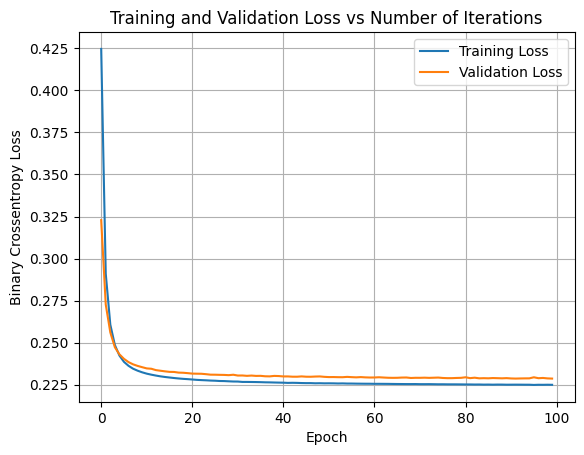
\includegraphics[scale=0.45]{appendix/b2-loss.png}
    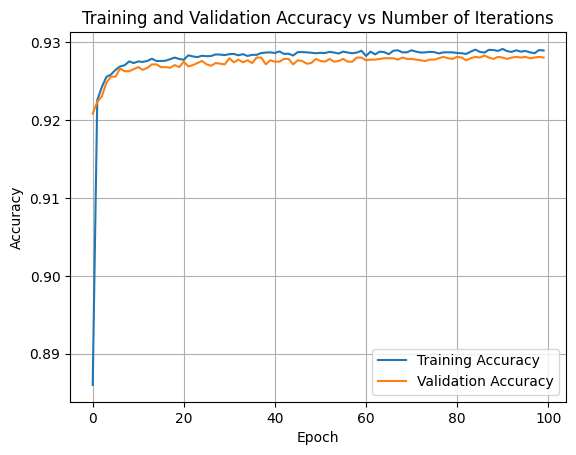
\includegraphics[scale=0.45]{appendix/b2-acc.png}
    \caption{Training and Validation Loss and Training and Validation Accuracy over 100 epochs using batch size = 32, learning rate $\alpha=0.05$, and L2 penalty $\lambda=0.001$.}
    \label{fig:epochs}
\end{figure} 
\section{Model diagnostics} \label{appendix:diagnostics}
Model checks and diagnostics for Model 0 (outlined in \ref{sec-mlmodel}) were performed using PyMC \cite{pymc}. Arviz was used to report Bayesian model analysis, including trace plots, R-hat plots, and posterior predictive checks \cite{arviz} \cite{mmm}. The posterior predictive checks displayed in Figure \ref{fig:ppc} show that model-generated data (inference data) is closely aligned with the observed data (2024 CES survey responses) \cite{arviz} \cite{mmm}. Figure \ref{fig:trace_plots} displays the trace plots for the intercept and weights. The trace plots show how the values of each weight change over time, with random fluctuations around a constant mean, indicating that the model has converged \cite{mmm}. Figure \ref{fig:rhat_plot} shows R-hat values very close to 1 and smaller than 1.01 for all predictors \cite{arviz}. This indicates that the chains mixed well and converged \cite{pymc} \cite{mmm}. Figure \ref{fig:plot_posterior} shows the posterior distribution of each model parameter \cite{arviz}.
\begin{figure}[H] 
    \centering
    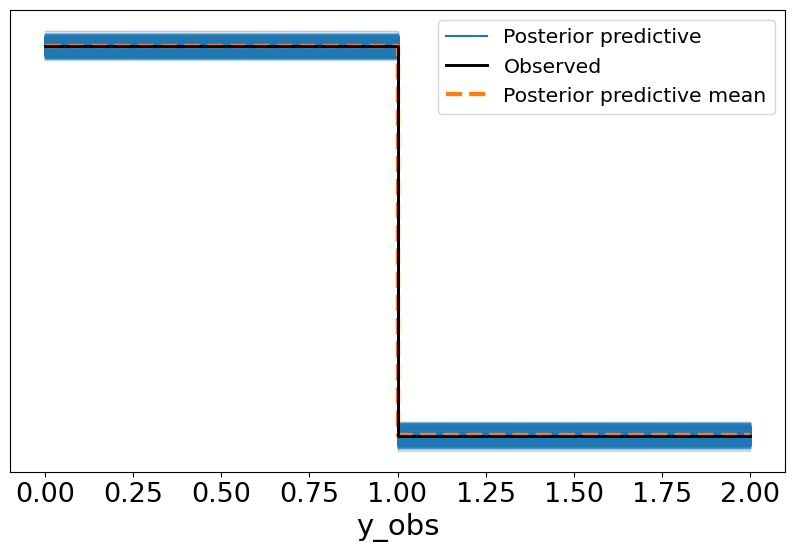
\includegraphics[scale=0.5]{appendix/ppcs.png}
    \caption{Posterior predictive checks}
    \label{fig:ppc}
\end{figure} 
\begin{figure}[H]
    \centering
    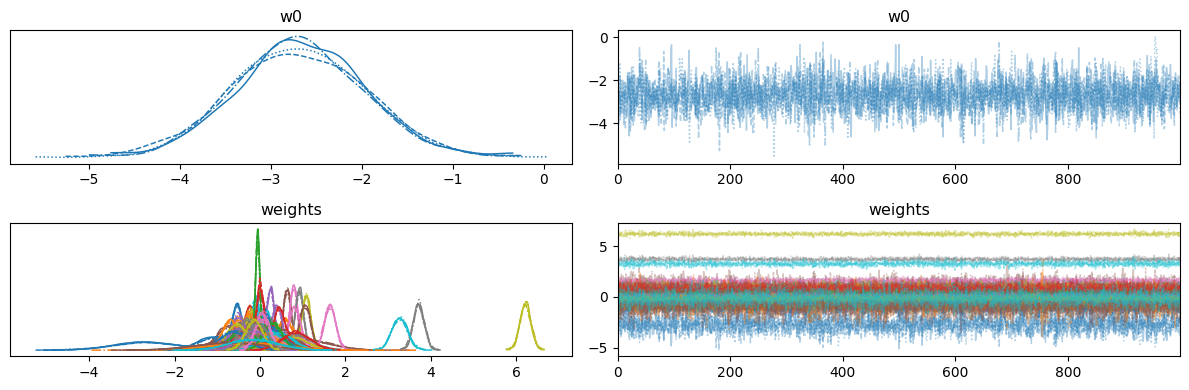
\includegraphics[scale=0.5]{appendix/trace_plots.png}
    \caption{Trace plots}
    \label{fig:trace_plots}
\end{figure} 
\begin{figure}[H]
    \centering
    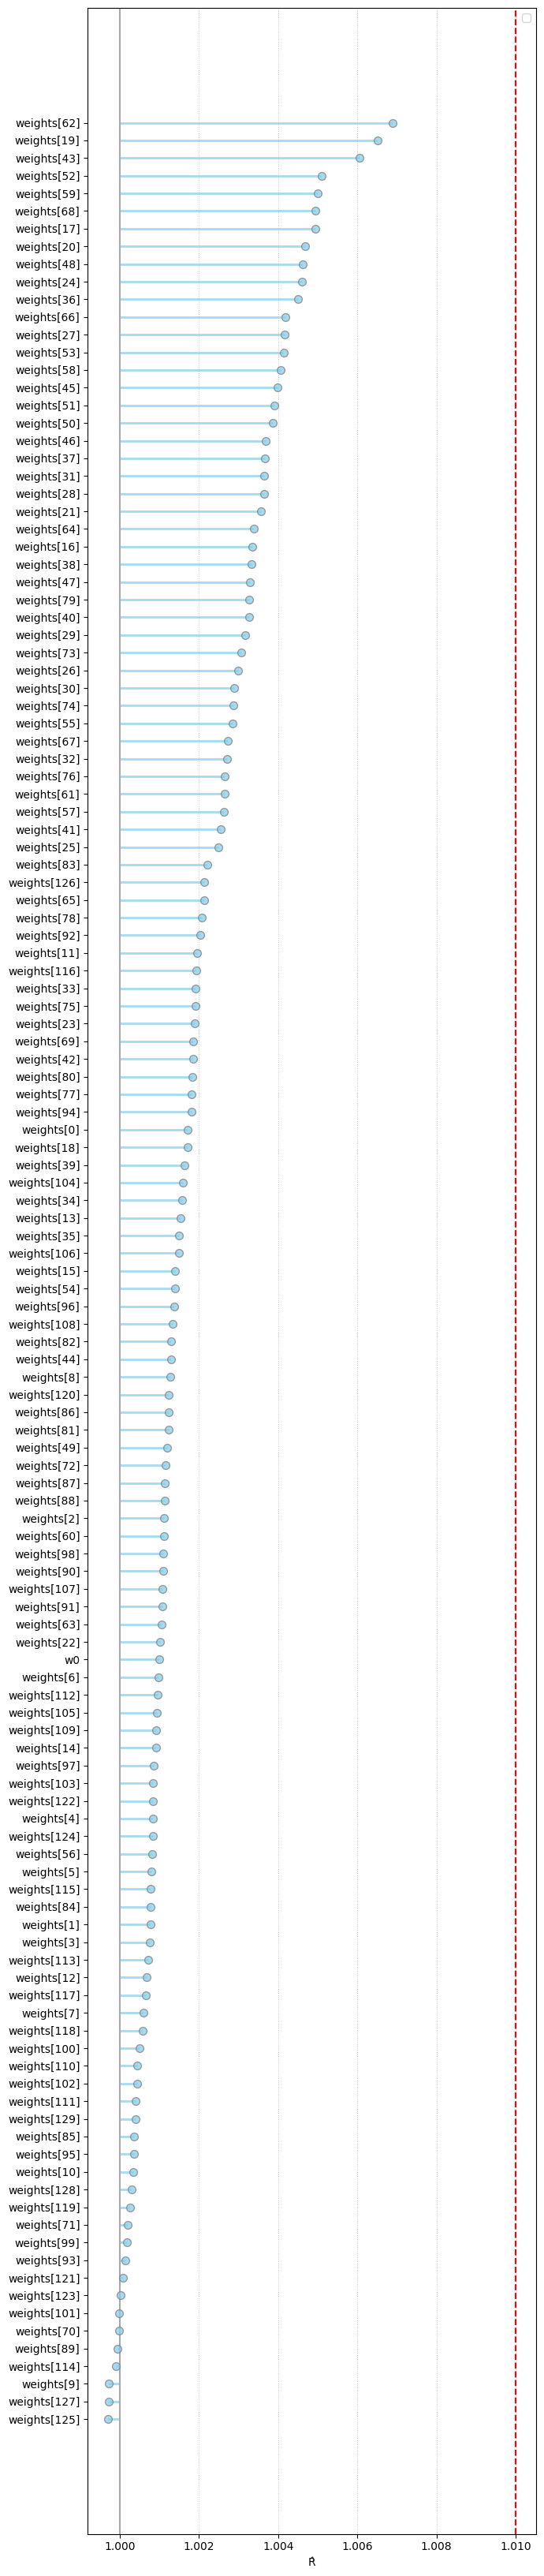
\includegraphics[scale=0.25]{appendix/rhat.png}
    \caption{R-hat plots}
    \label{fig:rhat_plot}
\end{figure} 
\begin{figure}[H]
    \centering
    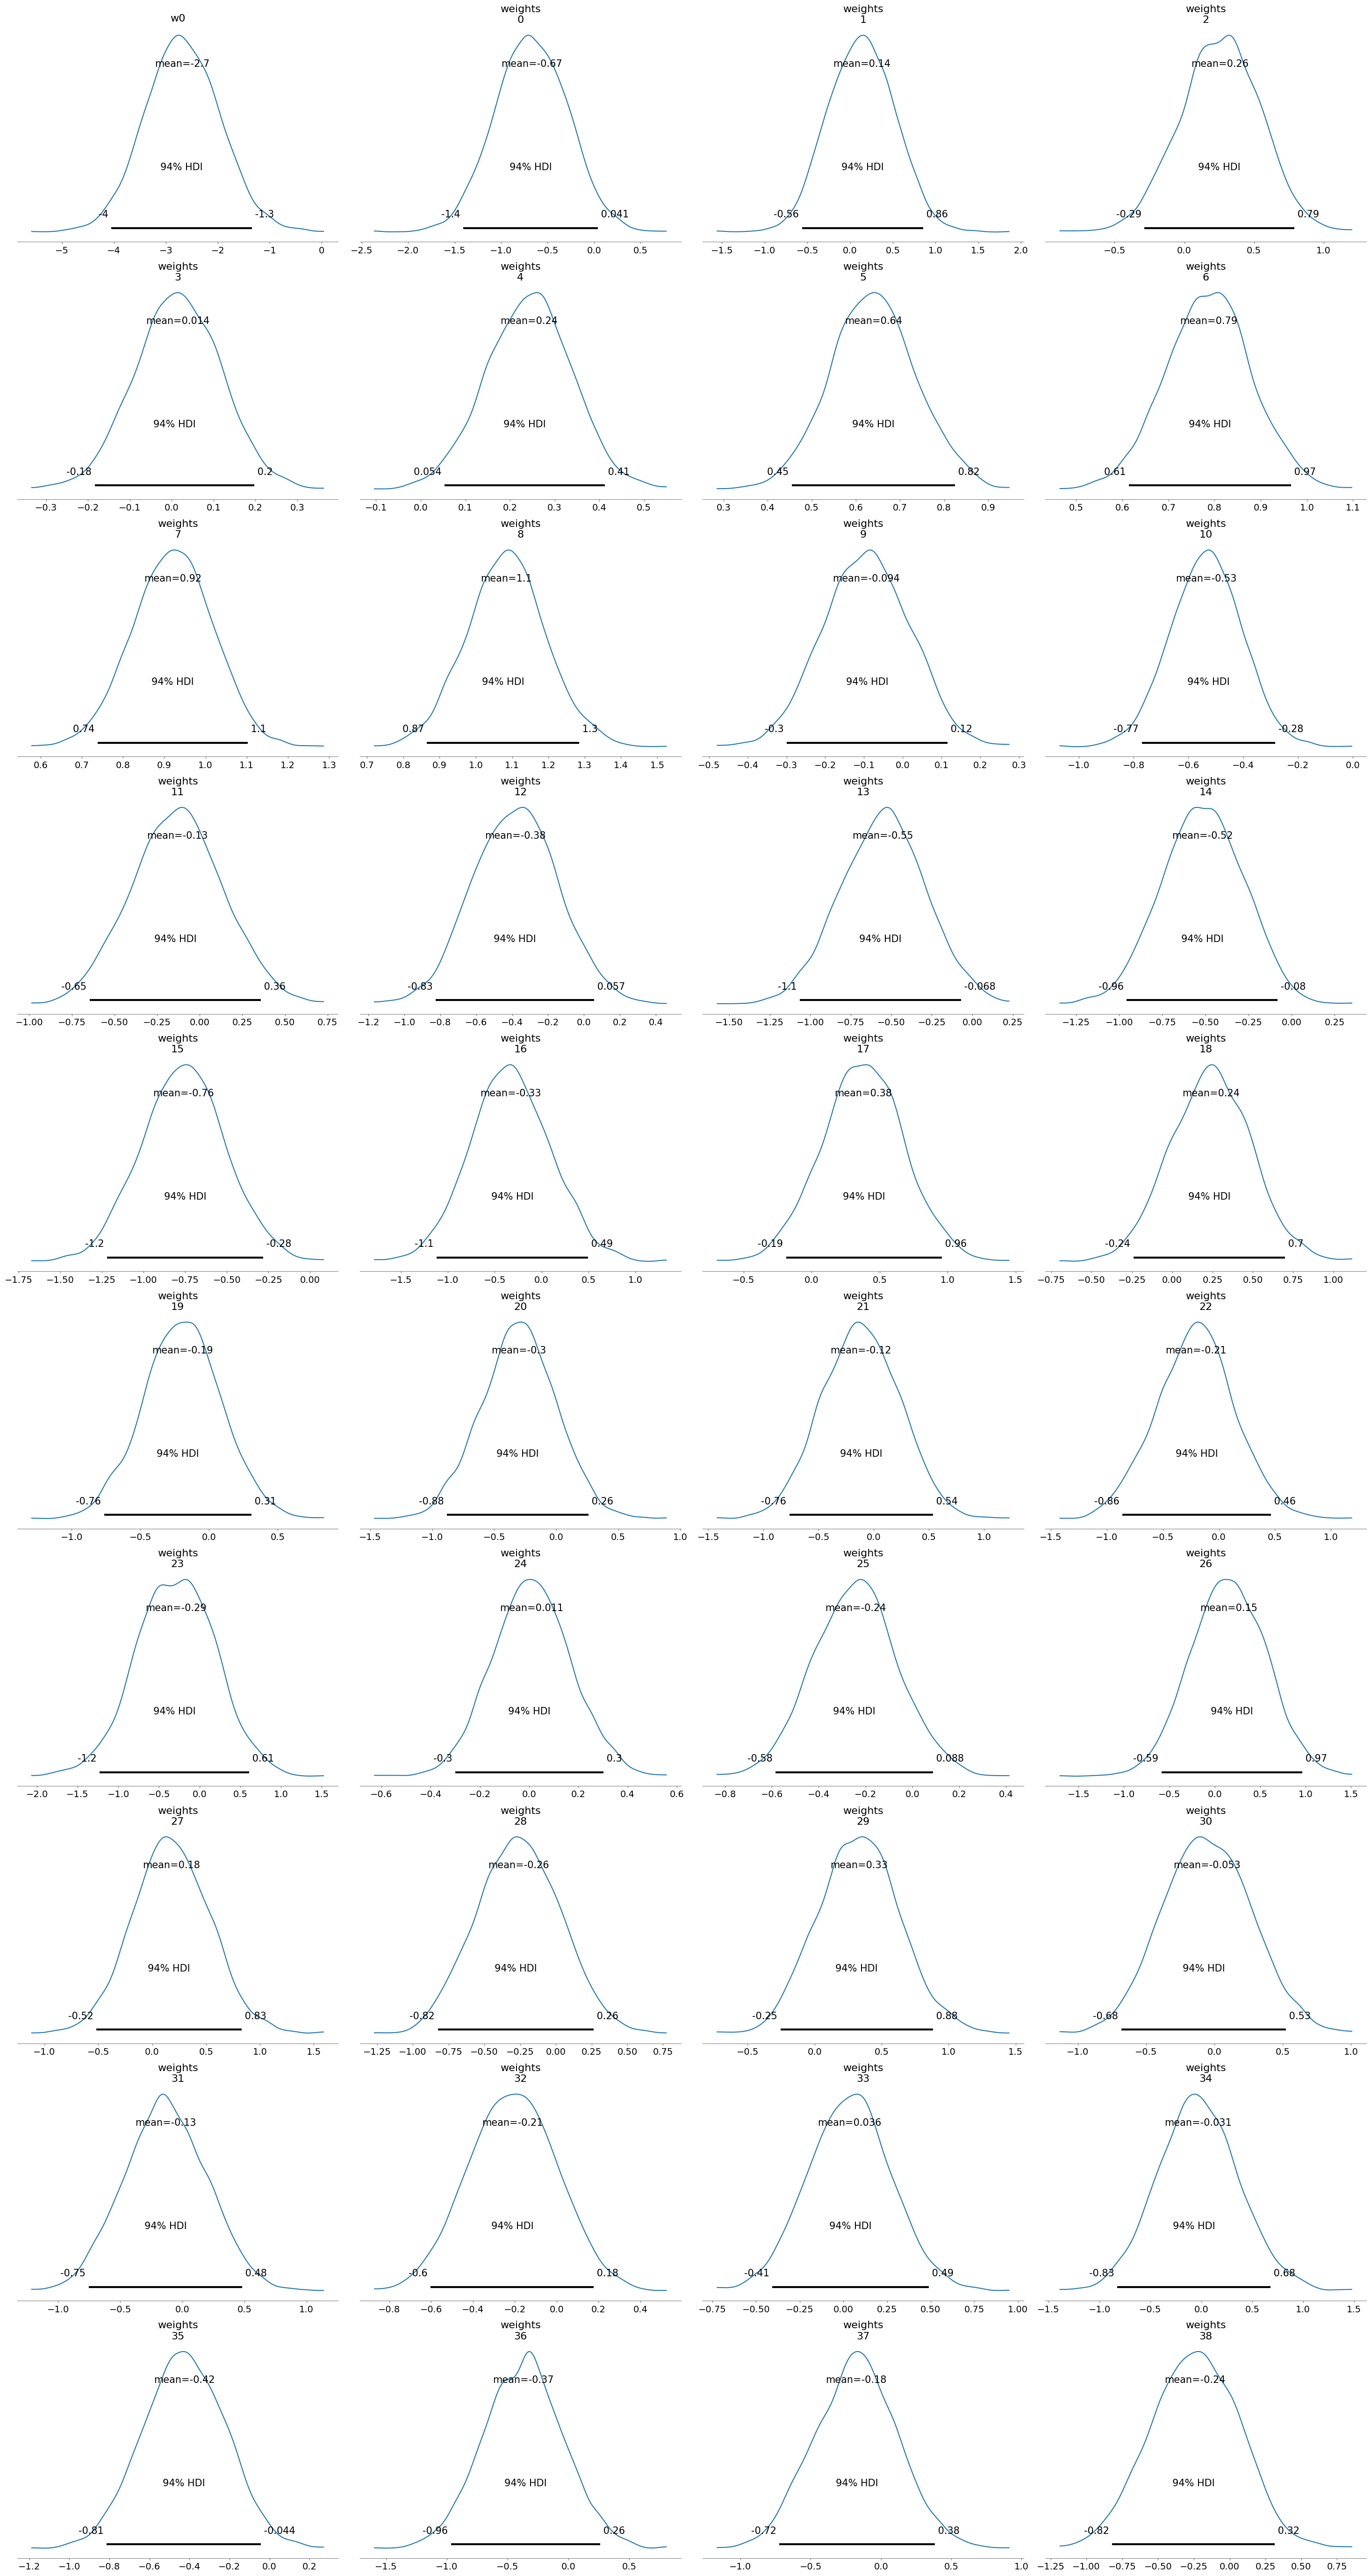
\includegraphics[scale=0.15]{appendix/posterior_plot.png}
    \caption{Posterior plots}
    \label{fig:plot_posterior}
\end{figure} 
\end{document}
